
% !TEX program = lualatex
% !TEX root = /Users/patricpf/Documents/repos/Bauschule-Baustoffe/HTg-26/Programm/KW_35_Programm.tex

% !TEX program = lualatex
\ifdefined\customoptions
    \documentclass[\customoptions]{beamer}
\else
    \documentclass[aspectratio=169,handout,12pt]{beamer}
\fi


\PassOptionsToPackage{dvipsnames,svgnames}{xcolor}

%\usepackage[utf8]{inputenc}
%\usepackage[ngerman]{babel} % Schweizer Rechtschreibung

\usepackage{polyglossia}
\setdefaultlanguage[variant = swiss]{german}
\usepackage{fontspec}
\setmainfont{Times New Roman}
\setsansfont{Arial}


\usepackage{amsmath}
\usepackage{siunitx}
\sisetup{
    locale = DE,
    inter-unit-product = \ensuremath{{\cdot}},
    detect-mode,             % Use the surrounding text font mode
    detect-family,           % Use the surrounding text font family
    detect-weight,           % Use the surrounding text font weight
    mode = text,             % Ensure that numbers and units are typeset in text mode
    %negative-powers = false, % Avoid using negative powers
    per-mode = symbol        % Use the division symbol for per units
}

\usepackage{tikz}
\usepackage{enumitem}
\usepackage{graphicx}
\usepackage{booktabs}
\usepackage{calc}
\usepackage{multicol}
\usepackage{amsmath}
\usepackage{fontawesome}
\usepackage{colortbl}


\usepackage{tcolorbox}
\tcbuselibrary{skins}

\usepackage[dvipsnames]{xcolor}

%\usepackage[scaled]{helvet} % Arial-ähnliche Schriftart (Helvetica)
%\renewcommand\familydefault{\sfdefault} % Setzt die Standard-Schriftart auf sans-serif


\usetheme{Madrid} % This theme is visually appealing
%\usecolortheme{whale} % A color theme with blue tones
\usecolortheme{dolphin} % A color theme with blue tones
\setbeamerfont{frametitle}{size=\Large}
\setbeamercolor{frametitle}{fg=blau_bauschule}
\setbeamercolor{toc}{fg=blau_bauschule}
\setbeamercolor{section in toc}{fg=blau_bauschule}
\setbeamercolor{subsection in toc}{fg=blau_bauschule}

\newcommand{\mylogo}{
    \begin{tikzpicture}[remember picture,overlay]
        \node[anchor=north east, yshift=-2mm, fill=white, inner sep=2pt] at (current page.north east) % Verschiebe das Logo um 5mm nach unten
        {
\includegraphics[height=0.4cm]{/Users/patricpf/Documents/repos/Bauschule-Baustoffe/template/bauschule-logo-5cm.png}}; % Grösse nach Bedarf anpassen
    \end{tikzpicture}
}

\logo{\mylogo}

\setbeamertemplate{headline}{%
    \begin{beamercolorbox}[wd=\textwidth,ht=0.5ex,dp=1ex]{upper separation line head}
    \end{beamercolorbox}
}

\setbeamercolor{upper separation line head}{bg=blau_bauschule}


% Anpassen des Frametitels, um ihn fett zu machen
\setbeamertemplate{frametitle}{%
    \nointerlineskip%
    \begin{beamercolorbox}[sep=0.3cm,left,wd=\paperwidth]{frametitle}%
        \usebeamerfont{frametitle}\bfseries\insertframetitle%
    \end{beamercolorbox}%
}

\setbeamertemplate{section in toc}[square]
\setbeamertemplate{subsection in toc}[square]

\newcommand{\BlueSectionSlide}{
    {
            \setbeamercolor{background canvas}{bg=blau_bauschule} % Temporarily set the background color
            \begin{frame}[plain] % Plain frame without navigation
                \begin{center}
                    {\Huge \color{white} \textbf{\insertsection}} % Section title in the center
                \end{center}
            \end{frame}
            \setbeamercolor{background canvas}{bg=} % Reset background color
        }
}

%\usebackgroundtemplate{
%    \includegraphics[width=\paperwidth,height=\paperheight]{my_pdf_copy_of_empty_ppt_template}
%}

% Setzen Sie hier den Namen des Fachs
\newcommand{\fachname}{Baustoffe}
\newcommand{\FinRes}[1]{\underline{\underline{#1}}}

\setbeamertemplate{footline}{%
    \begin{tikzpicture}[remember picture,overlay]
        % Dünner Farbverlauf
        \shade[left color=blau_bauschule, right color=blau_bauschule]
        ([yshift=0cm]current page.south west) rectangle ([yshift=0.5cm]current page.south east);
        % Autor linksbündig
        \node[anchor=south west, xshift=0.5cm, yshift=0.15cm] at (current page.south west) {%
            \textcolor{white}{\insertshortauthor}};
        % Titel zentriert
        \node[anchor=south, yshift=0.15cm] at (current page.south) {%
            \textcolor{white}{\fachname}};
        % Foliennummer rechtsbündig
        \node[anchor=south east, xshift=-0.5cm, yshift=0.15cm] at (current page.south east) {%
            \textcolor{white}{\insertframenumber{} / \inserttotalframenumber}};
    \end{tikzpicture}
}

%\setbeamertemplate{footline}{%
%  \hspace*{0.5cm}\textbf{\fachname}\hfill \insertframenumber / \inserttotalframenumber\hspace*{0.5cm}}

\setbeamerfont{block title}{size=\normalsize,series=\bfseries,family=\sffamily}
%\setbeamerfont{frametitle}{size=\LARGE,series=\bfseries,family=\sffamily}


\newtcolorbox{Merke}{
    enhanced,
    boxrule=0pt,frame hidden,
    borderline west={4pt}{0pt}{red!75!black},
    colback=white,
    sharp corners,
    before upper={\textbf{Merke:}\quad},
}

\newtcolorbox{Anwendungen}{
    enhanced,
    boxrule=0pt,frame hidden,
    borderline west={4pt}{0pt}{brown!75!black},
    colback=white,
    sharp corners
}




% Colors
\definecolor{blau_bauschule}{RGB}{22,65,148}
\setbeamercolor{frametitle}{fg=blau_bauschule}
\setbeamertemplate{navigation symbols}{} % Remove navigation symbols




\newtcolorbox{Definition_BS}[1]{
    enhanced,boxrule=1pt,
    colback=green!5!white,
    colframe=green!75!black,fonttitle=\bfseries, title = #1,
    %after title={\hfill\colorbox{black}{Definition}}
}



\newtcolorbox{Masseinheit}[1]{
    enhanced,
    boxrule=1pt,colframe=blue,
    colback=white,
    sharp corners,
    colframe=blue!75!black,
    title = #1,
    after title={\hfill\colorbox{blue}{Masseinheit}}
}


\newtcolorbox{myLösung}{
    enhanced,
    boxrule=1pt,
    colframe=gray!75!black, % Definiert die Farbe des Rahmens als dunkelgrau
    colback=gray!20, % Definiert die Hintergrundfarbe der Box als hellgrau
    %sharp corners, % Macht die Ecken der Box scharf (nicht abgerundet)
    title = {Lösung}, % Fest eingestellter Titel der Box
    after title={}, % Fügt das Label "Masseinheit" nach dem Titel hinzu
    coltitle=white, % Farbe des Titeltexts
    fonttitle=\bfseries % Schriftart des Titels
}


\newtcolorbox{myLernziele}{
    enhanced,
    colframe=cyan!75!black, % Rahmenfarbe (Türkis)
    colback=cyan!10, % Hintergrundfarbe (Helles Türkis)
    coltitle=black, % Titeltextfarbe (Schwarz)
    boxrule=1pt, % Rahmenstärke
    title={Lernziele}, % Fester Titel
    fonttitle=\bfseries, % Schriftart des Titels (Fett)
    left=2mm, % Innenabstand links
    right=2mm, % Innenabstand rechts
    top=1mm, % Innenabstand oben
    bottom=1mm % Innenabstand unten
}


\newtcolorbox{Fragenblock}{
    enhanced,
    colframe=orange!75!black, % Rahmenfarbe (Orange)
    colback=orange!10, % Hintergrundfarbe (Helles Orange)
    coltitle=black, % Titeltextfarbe
    boxrule=1pt, % Rahmenstärke
    title={Frage}, % Fester Titel
    fonttitle=\bfseries, % Schriftart des Titels (Fett)
    left=2mm, % Innenabstand links
    right=2mm, % Innenabstand rechts
    top=1mm, % Innenabstand oben
    bottom=1mm % Innenabstand unten
}

\newcommand{\folieFragen}{%
    \subsection{Fragen zur letzten Lektion}
    \begin{frame}{Fragen zur letzten Lektion}
        \begin{itemize}
            \item Haben Sie Fragen zur letzten Lektion?
        \end{itemize}

    \end{frame}
}

\newcommand{\naechstePruefung}[2]{%
    \subsection{Nächste Prüfung}
    \begin{frame}{Nächste Prüfung}
        \begin{itemize}
            \item[\textbullet] {\textbf{#1:}\hspace{5pt}}\textcolor{red}{\textbf{Prüfung:} #2}
        \end{itemize}
    \end{frame}
}

\newcommand{\pruefung}[3]{%
    \section{Prüfung}
    \BlueSectionSlide
    \begin{frame}{\textcolor{red}{Prüfung: #1}}
        \begin{itemize}
            \item[\textbullet] Bitte Namen eintragen:  \textit{Nachname Vorname}
            \item[\textbullet] Zeit: #2 Minuten
            \item[\textbullet] \href{#3}{\textcolor{blue}{Link zur Prüfung}}
        \end{itemize}
    \end{frame}
}

\newcommand{\Lernziele}[1]{%
    \begin{frame}{Lernziele}
        \begin{itemize}
            #1
        \end{itemize}
    \end{frame}
}


\newcommand{\notenverteilung}[5]{
    \begin{frame}{Notenverteilung}

        \begin{table}[h!]
            \centering
            \begin{tabular}{ll}
                \toprule
                \textbf{{}}              & \textbf{Note} \\ \midrule
                Minimum                  & #1            \\
                Median                   & #2            \\
                Mittelwert               & #3            \\
                Maximum                  & #4            \\
                Standardabweichung (Std) & #5            \\ \bottomrule
            \end{tabular}
        \end{table}
    \end{frame}
}

\newcommand{\notenformel}[3]{%
    \begin{frame}{Formel für die Notenberechnung}
        \begin{itemize}
            \item[\textbullet] Note 1 mit #1 Punkten
            \item[\textbullet] Note 6 mit #2 Punkten von maximal #3 Punkten
        \end{itemize}
    \end{frame}
}

% Set the title, author, and date
\title{\textbf{Lektionsprogramm HTg-26}}
\author{Patrick Pfändler}
\date{25.08.2025}


\begin{document}

\frame{\titlepage}


%\folieFragen



\begin{frame}{Inhalt der heutigen Lektion}
    \tableofcontents
\end{frame}


\section{Organisatorisches}
\BlueSectionSlide

\subsection{Uploads auf Teams}
\begin{frame}{Uploads auf Teams}
    \begin{itemize}
        %\item[\textbullet] Auswertung Prüfung
        %\item[\textbullet] Slides Beton Teil 1 (neue Version)
              %\item[\textbullet] Aktualisierter Terminplan
              %\item[\textbullet] Arbeitsauftrag Schmutziger Baustoff
        %\item[\textbullet] Mischungsberechnung: Aufgabenblatt und Folien (einfach und mittel)
        \item[\textbullet] Lernziele Prüfung
        %\item[\textbullet] Zusammenfassung Prüfungsstoff
        %\item[\textbullet] Unterlagen zu den Vorträgen
        %\item[\textbullet] Aufgabe zu Verdichtungsmass
        %\item[\textbullet] 06 Kunststoffe: Folien
        %\item[\textbullet] Lernziele Prüfung 3: Beil 1 \& 2 ton Te
        %\item[\textbullet] Vortrag Yanis
        %\item[\textbullet] Keine neuen Uploads diese Woche
        \item[\textbullet] Metalle: Folien
        \item[\textbullet] 99 Eidgenössische Prüfung
    \end{itemize}

\end{frame}


\section{Rückblick auf letzte Woche}
\BlueSectionSlide


\section{Padlet}
%\BlueSectionSlide
\begin{frame}{Padlet}
    \begin{itemize}
        \item[\textbullet] Ziel wäre es, Fragen zu den Themen zu sammeln, diese können dann in den nächsten Lektionen beantwortet oder als Quiz zur Prüfungsvorbereitung verwendet werden.
        \item[\textbullet] Link: \url{https://padlet.com/pfaendler/Fragen}
        \item[\textbullet] Ergänzung der Organisation nach Thema (in den Titeln)
    \end{itemize}
\end{frame}


\begin{frame}{Padlet ausfüllen}

    \begin{itemize}
        \item[\textbullet] Zeit: ca. 5 Minuten
    \end{itemize}

\end{frame}



\section{Dämmstoffe}
\BlueSectionSlide


\begin{frame}{Besprechung des Quiz}

\end{frame}


\begin{frame}{Einheit der Wärmeleitfähigkeit}
	\begin{Definition_BS}{Wärmeleitfähigkeit}
		Die Wärmeleitfähigkeit $\lambda$ ist eine Materialkonstante, die angibt, wie gut ein Material Wärme leitet. Sie wird in der Einheit \si{\watt\per\meter\per\kelvin} angegeben.
	\end{Definition_BS}
	\pause
	\begin{Beispiel}{Wärmeleitfähigkeit von einigen Materialien}
		\begin{itemize}
			\item[\textbullet] \textbf{Holz:} $\lambda = \SI{0.1}{\watt\per\meter\per\kelvin}$
			\item[\textbullet] \textbf{Beton:} $\lambda = \SI{1.5}{\watt\per\meter\per\kelvin}$
			\item[\textbullet] \textbf{Luft:} $\lambda = \SI{0.025}{\watt\per\meter\per\kelvin}$
		\end{itemize}
	\end{Beispiel}
\end{frame}

\begin{frame}{Steinwolle besteht aus:}
    \begin{Fragenblock}
        Steinwolle besteht aus:
        
        \begin{itemize}
            \item[\faSquare] künstlichen Mineralfasern
            \item[\faSquare] natürlichen Mineralfasern
        \end{itemize}
    \end{Fragenblock}
\end{frame}

\begin{frame}{Steinwolle besteht aus:}
    \begin{Fragenblock}
        Steinwolle besteht aus:
        
        \begin{itemize}
			\item[\textcolor{green!70!black}{\faCheckSquare}] künstlichen Mineralfasern
			\item[\faSquare] natürlichen Mineralfasern
        \end{itemize}
    \end{Fragenblock}
\end{frame}

\begin{frame}{Steinwolle ist resistent gegen Fäulnis?}
    \begin{Fragenblock}
        Steinwolle ist resistent gegen Fäulnis?
        
        \begin{itemize}
            \item[\faSquare] Richtig
            \item[\faSquare] Falsch
        \end{itemize}
    \end{Fragenblock}
\end{frame}

\begin{frame}{Steinwolle ist resistent gegen Fäulnis?}
    \begin{Fragenblock}
        Steinwolle ist resistent gegen Fäulnis?
        
        \begin{itemize}
			\item[\textcolor{green!70!black}{\faCheckSquare}] Richtig
			\item[\faSquare] Falsch
        \end{itemize}
    \end{Fragenblock}
\end{frame}


\begin{frame}{Glaswolle vs. Steinwolle}

	\begin{block}{Steinwolle}
		\ldots ist für gewöhnlich gelbgrün bis graugrün.
	\end{block}
	\pause
	\begin{block}{Glaswolle}
		\ldots zeigt eine gelbe, weisse oder braune Farbgebung auf.
	\end{block}
\end{frame}

\begin{frame}{Weisses Granulat}

    \begin{figure}[H]
        \centering
        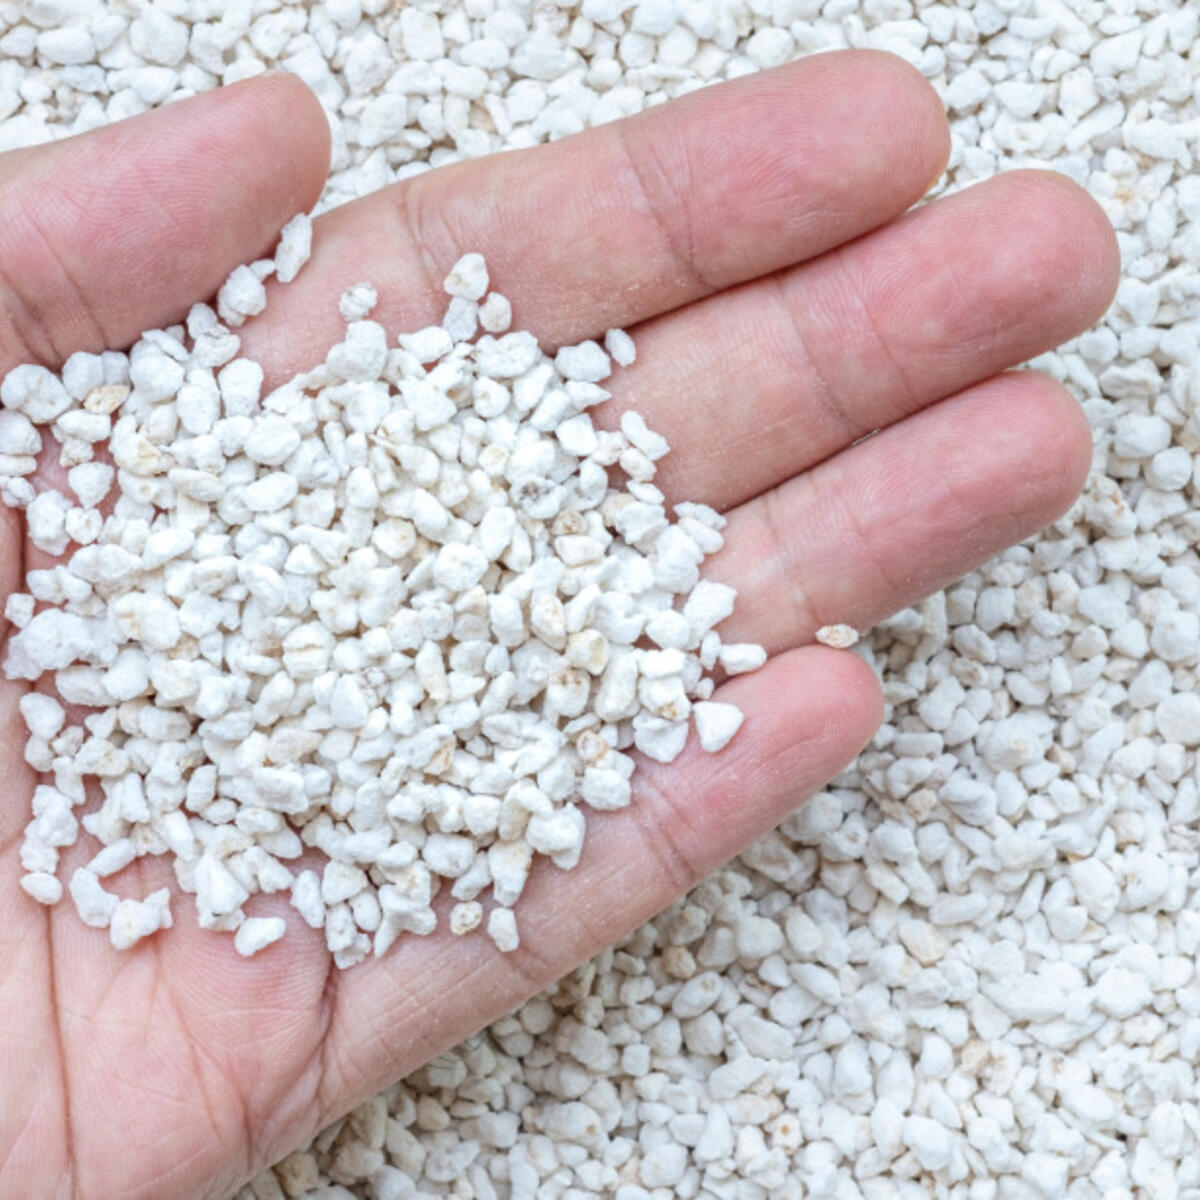
\includegraphics[height=0.7\textheight]{/Users/patricpf/Documents/repos/Bauschule-Baustoffe/Unterlagen/12_WDS/Bilder/Perlit.jpg}
        \caption{Perlit. (Styropor ist ein Markenname für Polystyrol und bereits eine Platte.)}
    \end{figure}


\end{frame}

\frageMitZweiFolien{Eigenschaften von Schurwolle}{Dämmstoffe aus Schurwolle haben eine hohe Speicherkapazität von Luftfeuchtigkeit.}{richtig}

\frageMitZweiFolien{Eigenschaften von Holzwollplatten}{Holzwollplatten sind bekannt als sehr guter Dämmstoff.}{falsch}

\frageMitZweiFolien{Zellulosefasern}{Isofloc ist ein bekanntes Produkt für Dämmstoffe aus Zellulosefasern.}{richtig}

\frageMitZweiFolien{Bindemitteln von Holzwollplatten}{Holzwollplatten werden i.d.R. mit Zement oder Gips gebunden.
}{richtig}

\frageMitZweiFolien{Eigenschaften von Holzfasterplatten}{Holzfaserplatten haben i.d.R. eine gute Wärme und ein gute Schalldämmung.
}{richtig}

\frageMitZweiFolien{Expansion von PS-Gries}{Das Polystyrolgries wird auf das ca. 20-fache seines Ausgangsvolumen aufgebläht.
}{falsch}

\frageMitZweiFolien{Produktname: Styrofoam}{Styrofoam ist ein XPS-Produkt.
}{richtig}


\begin{frame}{$\lambda$-Wert- Berechnungen}

	Bitte nochmals vor der Prüfung individuell anschauen.

\end{frame}



\section{Eidgenössische Prüfung}
\BlueSectionSlide
\begin{frame}{Wegleitung zur Eidgenössischen Prüfung}
    \begin{itemize}
        \item[\textbullet] Total 570 min Prüfung (schriftlich und mündlich)
        \item[\textbullet] 4 Prüfungsteile
    \end{itemize}
\end{frame}

\begin{frame}{Prüfungsteil 1: geleite Fallarbeit (180 min)}
    \begin{itemize}
        \item Teil 1: Bauprogramme und Ausführungs-konzepte erstellen
        \item Teil 2: Bedarf an Betriebsinventar und Baumaterial ermitteln
        \item Teil 3: Bedarf an Personal und Subunternehmen ermitteln
        \item Teil 4: Erschliessung, Einrichtung, Vermessung und Absteckung veranlassen/kontrollieren
    \end{itemize}
    \vspace{1em}
    $\Rightarrow$ Koordinieren in Bauprojekten
\end{frame}


\begin{frame}{Prüfungsteil 2: Geleitete Fallarbeit (120 min)}
    \begin{itemize}
        \item Teil 1: Bauausführung
        \item Teil 2: Leistungsdokumentation erstellen
    \end{itemize}
\end{frame}


\begin{frame}{Prüfungsteil 1 und 2}

\begin{myLernziele}
    In dieser Prüfungsform bearbeiten die Kandidat/innen verschiedene Teilaufgaben zu einem vielschichtigen Praxisfall. Die Teilaufgaben beziehen sich auf die Kernprozesse und -aufgaben des Berufs. Die Kandidat/innen werden in der geleiteten Fallarbeit systematisch mittels verschiedenen Teilaufgaben durch die Bearbeitung des Falls geführt.
    \vspace{1em}
    
    $\Rightarrow$ Überprüfung, ob Kandidat/innen analytische und konzeptionelle Kompetenzen besitzen und in ganz konkreten beruflichen Situationen ihre Kompetenzen umsetzen können.
\end{myLernziele}

\end{frame}

\begin{frame}{Prüfungsteil 3: Kleine Fallbeschreibungen und Handlungssimulationen (180 min)}
    \begin{itemize}
        \item Fokus kleine Fallbeschreibungen: Analyse und Vorgehen
        \item Fokus Handlungssimulationen: Korrekte und vollständige Umsetzung einer Handlung in konkreten und in sich abgeschlossenen Routinesituationen
        \item[\textbullet] 4 bis 6 Fallbeschreibungen
        \item[\textbullet] 2 bis 4 Handlungssimulationen
    \end{itemize}
        \vspace{1em}
    $\Rightarrow$ Zusammenarbeiten, Führen und Umsetzen von Akquisitions- und Managementaufgaben”
\end{frame}


\begin{frame}{Prüfungsteil 1 und 2}

\begin{myLernziele}
Kleine Fallbeschreibungen (auch Mini-Cases MC) sind eine Prüfungsform, in welcher kurze Beschreibungen von praktischen Situationen im Hinblick auf das berufliche Handeln analysiert werden. Die Kandidat/innen setzen sich sowohl mit der Situation als auch mit dem möglichen Vorgehen in der Situation auseinander. Dabei nehmen sie eine bestimmte Rolle ein.
    \vspace{1em}

    $\Rightarrow$ Überprüfung, ob Kandidat/innen die Situation oder das rollenkonforme Verhalten in einer Situation einschätzen können;  aus den Situationen Schlüsse und Konsequenzen für das Handeln ableiten können; vorzunehmende Handlungen aufzeigen können.
\end{myLernziele}

\end{frame}




\begin{frame}{Prüfungsteil 4: Überzeugen in seiner beruflichen Schnittstellenfunktion (90 min)}
    \begin{itemize}
        \item 4.1 Reflexionsgespräch (60 min, inkl. 30 min Vorbereitung)
        \item \begin{itemize}
            \item Teil 1: 1 Vorgegebene Praxissituation bearbeiten 
            \item Teil 2: 2 Eigene Praxisfalle analysieren \& Massnahmen/Schlussfolgerungen für das Handeln ableiten
        \end{itemize}
        \item 4.2 Erfolgskritische Situationen (30 min)
        \begin{itemize}
            \item Im Team agieren (HKB C)
            \item Anspruchsgruppen beraten und betreuen (HKB C)
            \item MA-Gespräche führen (HKB D) etc.
            \item 4 - 6 Erfolgskritische Situationen kommunikativ
        \end{itemize}
    \end{itemize}
\end{frame}



\begin{frame}{4.1 Reflexionsgespräch (mündlich)}
    \textbf{Definition} \\
    In einem Reflexionsgespräch reflektieren die Kandidatinnen und Kandidaten ihre berufliche Rolle und ihr Verhalten ausgehend von vorgegebenen Praxissituationen sowie von eigenen Praxisfällen. Sie erkennen die Problemstellungen und leiten geeignete Massnahmen für das eigene Handeln ab.
\vspace{1em}



    \begin{myLernziele}
        Überprüfung, ob Kandidat/innen
\begin{itemize}
    \item[\textbullet]  ihre Rolle in beruflichen Situationen analysieren und reflektieren können
    \item[\textbullet]  plausible Vorgehensweisen, Alternativen und Massnahmen ableiten können
\end{itemize}
\end{myLernziele}

\end{frame}


\begin{frame}{4.2 Erfolgskritische Situation kommunikativ }
    \textbf{Definition} \\
Eine Erfolgskritische Situation beschreibt eine praxisnahe und schwierige Arbeitssituation, in der es in besonderem Mass darauf ankommt, dass der/die Kandidat/in kompetent handelt. Ein Critical Incident (CI) kommunikativ beschreibt eine anspruchsvolle Kommunikationssituation, in der es in besonderem Mass darauf ankommt, dass der/die Kandidat/in kompetent kommuniziert. Nicht nur das «WAS» seiner/ihrer Aussagen spielt eine Rolle, sondern vor allem die Art und Weise «WIE» er/sie diese vorbringt. Der Einsatz von Kommunikationstechniken ist zentral.

    \begin{myLernziele}
        Überprüfung, ob Kandidat/innen
\begin{itemize}
    \item[\textbullet]  Anspruchsvolle Kommunikationssituationen - allenfalls unter Zeitdruck situationsgerecht bewältigen können.
\end{itemize}   
\end{myLernziele}

\end{frame}


\begin{frame}{Ausblick vom SBV (i)}

\textbf{Definition: Handlungskompetenz}\\
«Kompetenz ist eine Disposition, die Personen befähigt, bestimmte Arten von Problemen erfolgreich zu lösen, also konkrete Anforderungssituationen eines bestimmten Typs zu bewältigen.
Die berufliche Handlungskompetenz ist die Fähigkeit einer Person, eine berufliche Tätigkeit erfolgreich auszuüben, indem sie ihre eigenen Selbst, Methoden-, Fach- und Sozialkompetenzen nutzt.»
\footnote{Definition SBFI (Staatssekretariat für Bildung, Forschung und Innovation), 2020}
\vspace{1em}

«Die Bereitschaft und Befähigung des Einzelnen sich in beruflichen, gesellschaftlichen und privaten Situationen sachgerecht sowie individuell und sozial verantwortlich zu verhalten.»
\footnote{Abgeleitete Definition der Prüfungskommission}

\end{frame}

\begin{frame}{Ausblick vom SBV (ii)}
\begin{itemize}
    \item[\textbullet] An der Bauführerprüfung wird nicht nur Wissen abgefragt, sondern es werden praxisnahe Aufgaben gestellt. Dafür braucht es eine Portion Erfahrung. $\Rightarrow$ Haben Sie noch Lücken, schliessen Sie diese rechtzeitig und tauschen Sie sich mit erfahrenen Kollegen aus (Holschuld!).
    \item[\textbullet] Die Aufgaben sind anspruchsvoll und zielen auf die Schnittstellenfunktion ab, also \emph{fächerübergreifend} und \emph{vernetzt}.
    \item[\textbullet] Für die erfolgreiche Bearbeitung der Aufgaben braucht es neben der Handlungskompetenz, auch Fachkompetenz, Sozialkompetenz, Selbstkompetenz und Methodenkompetenz.
\end{itemize}
\end{frame}




\section{Vorträge}
\BlueSectionSlide

\begin{frame}{Vorträge}
    \begin{itemize}
        \item[\textbullet] Vorträge von den Schülern
        \item[\textbullet] 7 bis 15 Minuten pro Vortrag
        \item[\textbullet] 5 Minuten Fragen
        \item[\textbullet] Folien sind auf Teams hochgeladen
    \end{itemize}
\end{frame}

\subsection{Vortrag: Emanuel}
\begin{frame}{Fassadenaufbau mineralisch}
    von Emanuel Banicin
\end{frame}

\subsection{Vortrag: Bruno}
\begin{frame}{richtige Mörtel im Umgang mit Naturstein}
    von Bruno Kuster
\end{frame}










\section{Metalle}
\BlueSectionSlide

\begin{frame}{Metalle}
\begin{itemize}
    \item[\textbullet] Einführung in die Metalle
\end{itemize}
\end{frame}






\section{Organisatorisches}
\BlueSectionSlide



% \begin{frame}{Fragen zur Prüfung?}

% \end{frame}



\begin{frame}{Ausblick auf die nächste Lektion}
\begin{itemize}
    \item[\textbullet] Wärmedämmstoffe Abschluss 
    \item[\textbullet] Weitere Vorträge
\end{itemize}
\end{frame}

\naechstePruefung{08.09.2025}{Kunststoffe, Dämmstoffe und Innovation}


\end{document}